\documentclass{article}

\usepackage[final]{neurips_2022}

\usepackage[utf8]{inputenc} % allow utf-8 input
\usepackage[T1]{fontenc}    % use 8-bit T1 fonts
\usepackage{hyperref}       % hyperlinks
\usepackage{url}            % simple URL typesetting
\usepackage{booktabs}       % professional-quality tables
\usepackage{amsfonts}       % blackboard math symbols
\usepackage{nicefrac}       % compact symbols for 1/2, etc.
\usepackage{microtype}      % microtypography
\usepackage{xcolor}         % colors
\usepackage{graphicx}
\usepackage[font=small,labelfont=bf]{caption} % Required for specifying captions to tables and figures

\usepackage{algpseudocode}
\usepackage{algorithm}
\usepackage{amsmath}
\usepackage{amsthm,amsfonts,dsfont}
\usepackage{amssymb,latexsym,graphicx,multirow,multicol}
\usepackage{mathtools}
\usepackage{hyperref}
\usepackage{xcolor}
\usepackage{pdfpages}
\usepackage{soul}
\usepackage[thinc]{esdiff}
\hypersetup{
	colorlinks,
	linkcolor={red!75!black},
	citecolor={blue!75!black},
	urlcolor={blue!75!black}
}

\newtheorem{theorem}{Theorem}[section]
\newtheorem*{thm}{Theorem}
\newtheorem*{conj}{Conjecture}
\newtheorem*{remark}{Remark}
\newtheorem{proposition}[theorem]{Proposition}
\newtheorem{lemma}[theorem]{Lemma}
\newtheorem{conjecture}[theorem]{Conjecture}
\newtheorem{claim}[theorem]{Claim}
\newtheorem{fact}[theorem]{Fact}
\newtheorem{example}[theorem]{Example}
\newtheorem{corollary}[theorem]{Corollary}
\newtheorem{definition}{Definition}

\newcommand{\C}{\ensuremath{\mathbb{C}}}
\newcommand{\N}{\ensuremath{\mathbb{N}}}
\newcommand{\F}{\ensuremath{\mathbb{F}}}
\newcommand{\R}{\ensuremath{\mathbb{R}}}
\newcommand{\Z}{\ensuremath{\mathbb{Z}}}
\newcommand{\prob}{\ensuremath{\mathbb{P}}}
\newcommand{\Q}{\mathbb{Q}}

\newcommand{\GL}{\ensuremath{\text{GL}}}
\newcommand{\sign}{\ensuremath{\text{sign}}}
\newcommand{\lat}{\mathcal{L}}
\newcommand{\M}{\mathcal{M}}
\newcommand{\NN}{\mathcal{N}}
\newcommand{\V}{\mathcal{V}}
\newcommand{\pv}{\mathcal{P}}

\newcommand{\eps}{\varepsilon} 
\renewcommand{\epsilon}{\varepsilon}
\newcommand{\poly}{\mathrm{poly}}
\newcommand{\polylog}{\mathrm{poly\,log}}
\DeclareMathOperator{\negl}{negl}
\newcommand{\grad}{\nabla}
\newcommand{\rank}{\mathrm{rank}}
\newcommand{\vol}{\mathrm{vol}}
\newcommand{\view}{\mathrm{view}}
\newcommand{\err}{\mathrm{err}}
\newcommand{\Var}{\mathrm{Var}}
\newcommand{\Gen}{\mathrm{Gen}}
\newcommand{\Enc}{\mathrm{Enc}}
\newcommand{\Dec}{\mathrm{Dec}}
\newcommand{\Sign}{\mathrm{Sign}}
\newcommand{\Ver}{\mathrm{Ver}}
\newcommand{\Com}{\mathrm{Com}}
\DeclareMathOperator*{\argmax}{arg\,max}
\DeclareMathOperator*{\argmin}{arg\,min}
\DeclareMathOperator*{\E}{\mathbb{E}}
\DeclareMathOperator{\dist}{dist}
\DeclareMathOperator{\spn}{span}
\newcommand{\intd}{\, {\rm d}}

\renewcommand{\vec}[1]{\ensuremath{\boldsymbol{#1}}}
\newcommand{\basis}{\ensuremath{\mathbf{B}}}
\newcommand{\gs}[1]{\ensuremath{\widetilde{\vec{#1}}}}
\newcommand{\tre}{\trianglerighteq}
\newcommand{\tr}{\triangleright}
\newcommand{\tle}{\trianglelefteq}
\newcommand{\tl}{\triangleleft}
\newcommand{\tlast}{t_{\text{last}}}
\newcommand{\A}{\mathcal{A}}
\newcommand{\B}{\mathcal{B}}

% inner product
\DeclarePairedDelimiter\inner{\langle}{\rangle}
% rounding off
\DeclarePairedDelimiter\round{\lfloor}{\rceil}
% floor function
\DeclarePairedDelimiter\floor{\lfloor}{\rfloor}
% ceiling function
\DeclarePairedDelimiter\ceil{\lceil}{\rceil}
% length of some vector, element
\DeclarePairedDelimiter\length{\lVert}{\rVert}

\title{Safety Guarantees for Model Based Reinforcement Learning - Survey of a Control Barrier Function Approach}


\author{%
  Sahil Fatehpuria \\
  \texttt{sf382@cornell.edu} \\
}


\begin{document}


\maketitle

\begin{abstract}
Reinforcement learning systems have wide potential applications to high risk systems that run in the real world. However, when working with theses systems that, if the expected performance is not achieved, may lead to serious safety concerns for the people around the system. Thus, for such systems, there is a need for some guarantees of performance, or at least assurance that some worst case scenarios can be avoided. One way this can be done is through the use of CBFs (Control Barrier Functions). We survey the existing research on this topic and try and provide a formal analysis of the expected learning guarantees when using this method. We focus mainly to the application to model based learning
\end{abstract}


\section{Introduction}

Reinforcement learning, in the past few years especially, has progressed in leaps and bounds. The potential for seemingly miraculous performance has even reached the attention of the broader public through applications like OpenAI's ChatGPT. However, despite this advancement in the field, reinforcement learning remains very much in the fledgling stage when it comes to being used for physical systems, 'in the real world' so to say. This is perhaps most noticeable in the world of autonomous vehicles, which seems to be one of the most natural applications of reinforcement learning. However, despite this, those working in the field have faced significant challenges in translating this theoretical application into real implementation \cite{kiran2021deep} One major roadblock is the question of safety. While this is obvious in the scenario of driverless cars that are interacting with humans and have the potential of endangering life and injury, it is relevant in any physical system, as a mistake caused by the learning process can translate into damage, which can halt the learning process and can be expensive to fix. One would expect this to be especially difficult to avoid for reinforcement learning algorithms, because of the inherent need for exploration. In the initial stages of learning, the algorithm needs to explore different option based on limited understanding of the world in order to better inform future decisions. However, during this process, it is hard to know whether an action is unsafe. Thus, it is clear that the question of safety for reinforcement learning is both important and challenging to answer. As a result, a lot of research has been done in this field through a variety of approaches, including things like changing the objective function to incorporate risk minimization, or giving instructions through an external 'teacher' \cite{garcia2015comprehensive}. One method that has gained traction recently comes from the intersection between reinforcement learning and control systems - Control Barrier Functions. In this report, I will give an overview of the current state on how Control Barrier Functions are used for safe reinforcement learning. We will cover some background, formalizing the concept of safety and explaining what a control barrier function is, look at the work that has been done into using control barrier functions for model free reinforcement learning, and then delve into the more complex model-based setting and see how control barrier functions can be adapted to provide safety guarantees there.
\newpage
\section{Background}
Control Barrier Functions are a concept developed for control systems. Thus, for the purpose of this survey, we will move away from the Markov Decision Process we typically use as the setting for reinforcement learning. Instead we will be trying to learn a dynamical system. At it's most basic, this is denoted by $\dot{x} = f(u; x)$ for $x \in \R^n$ and some function $f: \R^n \rightarrow \R^n$. Here, $x$ represents the current state of the system, and $\dot{x}$ represents the future state. $u \in \R^p$ represents control policy inputs, that we can change to get $\dot{x}$ to be what we desire. In the MDP setting, our policy chooses actions based on what it knows about the transition function. Similarly, here our policy would use what it knows about $f$ to choose $u$. With this setting, we can formally define what safety means for a dynamical system. Suppose we define a \textit{safe} set $C$ using a function $h$ such that $C = \{x : h(x) \geq 0\}$ Then, the dynamic system is deemed to be safe over $C$ if $C$ is forward invariant. That is, if our system starts in $x_0 \in C$ then $\dot{x} \in C$ (Note, this abstracts away some detail and rigor specific to dynamical systems, but is sufficient for our discussion). Control Barrier Functions are then choices of $h$ so that $C$ is guaranteed to be safe for a system. \\
We can see an explicit example of Control Barrier Functions \cite{ames2019control}, Let us examine a nonlinear affine control system, defined as $\dot{x} = f(x) + g(x)u$ for locally Lipschitz $f$ and $g$ and control inputs $u$. In this setting, we can come up with a necessary and sufficient condition on $h$ for the system to be safe on the set $C$ defined using $h$ as above. To do this, we need to first define a $K_\infty$ function. A function $\alpha : \R \rightarrow \R$ is said to be $K_\infty$ if $\alpha(0) = 0$ and it is strictly increasing. Denote by $L_f$ and $L_g$ the Lipschitz constants of $f$ and $g$. Then, $h$ is said to be a CBF if there exists a $K_\infty$ function $\alpha$ such that \begin{equation}
    \sup_u [L_fh(x) + L_gh(x)u] \geq -\alpha(h(x))
\end{equation} If $h$ satisfies these conditions, and if we only choose $u$ so that $L_fh(x) + L_gh(x)u \geq -\alpha(h(x))$ then we are guaranteed to never leave the safe set $C$ making it forward invariant. Further, if $C$ is forward invariant for some defined function $u = k(x)$ then the $h$ it is based on must be a CBF. In fact, this CBF provides an even more robust guarantee on the system - in that it makes $C$ asymptotically stable, which means that not only are we guaranteed to stay in $C$, if real world noise pushes the system slightly out of $C$, the system will be forced back into $C$ \cite{ames2016control} This makes it very easy to appy to real world settings. With the concept of control barrier function's established, and having taken a look at the powerful results that can be achieved by using them, we are now ready to look at their impact on the world of reinforcement learning.
\section{CBFs for model free learning}
The first attempt to integrate CBFs to provide safety for reinforcement learning was one in the setting of model free RL, by Cheng et al. in 2019 \cite{cheng2019end}. They came up with a way to integrate CBFs with existing model free learning algorithms to account for safety considerations. This allowed them to just adapt the best available algorithms, which are already well recognized, and just adapt them to consider safety as well. An additional advantage of their method was that it actually increased the efficiency of the exploration process. \\
The basic idea behind their process was to modify policy gradient RL methods and incorporate CBFs. They use simple RL to come up with a policy, and then use the CBF condition to project that policy into one that satisfies the constraint required to remain within the safe set. Effectively, the CBF defines the set of safe policies, and whatever policy the standard algorithm selects, the CBF condition is used to select the policy most similar to that one from within the safe set. This process is illustrated by the below workflow.\\
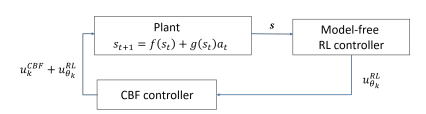
\includegraphics[scale = 1.5]{Screenshot 2023-05-13 180156.png}\\\\\\
They called this algorithm - CBF-Based Compensating Control with Reinforcement Learning. Note that a controller here refers to a sample of a learned policy. In the above figure, the plant refers to the model, which passes the current state $s$ to the RL controller - $u_{\theta_k}^{RL}(s)$ which is a function that takes in a state and outputs an action designed to maximize reward. The CBF controller - $u_k^{CBF}$ takes this action, as well as the current state, and intervenes as little as possible to make sure that the outputted action keeps the system in a safe state. This process is repeated over the time steps to iteratively come to the safe, optimum policy. As we can see, with this setup, the CBF controller is not involved in exploration at all. All of that is done by the standard RL algorithm, and the CBF only gets involved after that to ensure safety. While this is still useful, it discards the potential for the CBF technique to inform exploration itself, which would allow the focus of exploration to be on safe policies by itself, and thus improve efficiency. To take this into account, they came up with a second process based on the same concept: CBF-Based Guiding Control with Reinforcement Learning. This is illustrated in the below diagram: \\
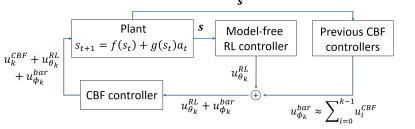
\includegraphics[scale = 1.5]{Screenshot 2023-05-13 180227.png}\\\\
The key difference here is the consideration of previous CBF controllers. Thus, now, at each time step we do not only use the RL algorithm to provide the controller that chooses the initial action. Instead, we use the CBF controllers that we had come up with in previous time steps in conjunction with the controller informed by the policy gradient iteration. This allows us to use the previously found safe policy as the starting point, instead of just always fixing updates made by the RL algorithm. Note that we still incorporate the RL method, because it is what actually aims for optimization, but because of this we still need to apply a CBF controller finally, because there is potential of being pushed outside the safe set. The below graphic from the paper illustrates the difference between compensating vs guided exploration:
\begin{center}
    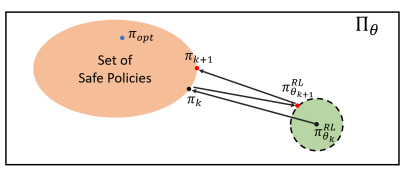
\includegraphics[scale = 1.1]{Screenshot 2023-05-13 184059.png} \\ 
    Above: Compensating Control\\
    Below: Guided Control\\ 
    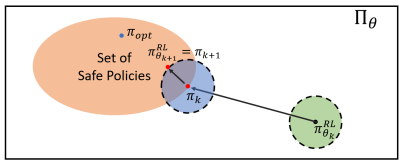
\includegraphics[scale = 1.1]{Screenshot 2023-05-13 184109.png} \\
\end{center}
The safety guarantees that this model achieves are based on the fact that the authors use a Gaussian Processes based model, which is the same as the one used in the model-based architecture that we will look at next, and so will be discussed in more detail there. The authors incorporated this technique with two premiere model-free RL algorithms: trust region policy optimization (TRPO) \cite{schulman2015trust} and deep deterministic policy gradients (DDPG) \cite{lillicrap2015continuous} to develop the algorithms denoted TRPO-CBF and DDPG-CBF. They then tested their resulting safe algorithms and got very successful results, as depicted in the figures below. These graphs show performance of the algorithms on the inverted pendulum environment from OpenAI \\
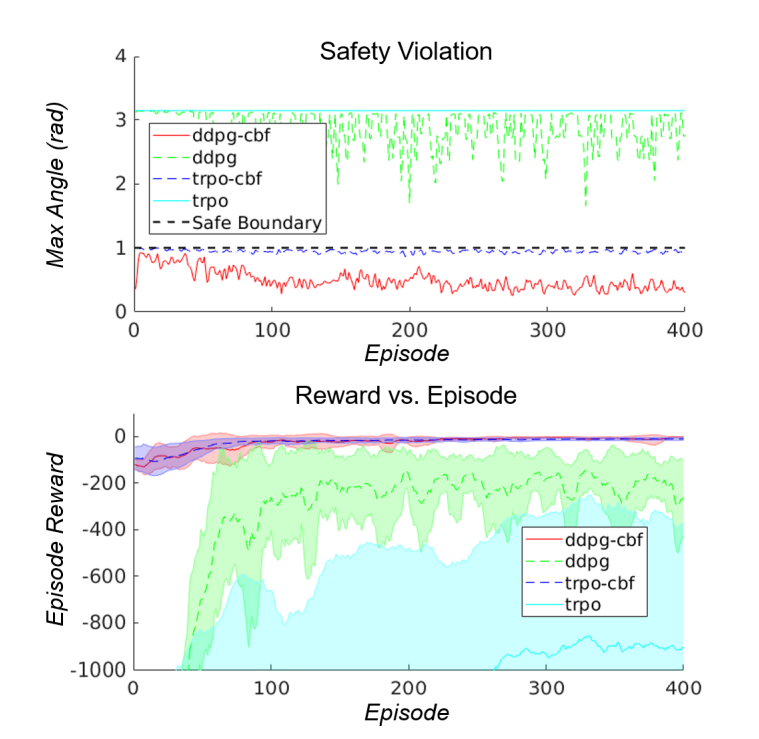
\includegraphics[scale = 0.9]{Screenshot 2023-05-13 200345.png}
As we can see, not only do both implementations stay almost entirely shy of the safe boundary, they receive consistently better rewards than their unsafe counterparts, and start performing well, in comparison to the unsafe methods, from the very first episode.
\section{CBFs for Model Based Learning}
The world of safe reinforcement learning is a rapidly evolving field, and one of the recent innovations is the extension of these CBF based methods to model-based problem architectures. The model based setting gives us more initial information to work with, in the form of a probabilistic understanding of the world through a model of the environment. As a result, one would expect CBFs to be very useful in employing that knowledge to come with a safe algorithm. That said, the model introduces an extra facet of uncertainty, which makes it more complex to provide probability bounds on safety that are needed to ensure confidence.\\
Some of the first work in this field was the paper by Zhang et al presented in 2021 \cite{zhang2021model}. We will take an in depth look at the approach, safety guarantees, and results achieved by the paper. 
\subsection{Problem Setup}
The dynamic system we will be working with is slightly different from the one we defined the CBF on in the background section. Here, we work with discrete time, and our non-linear system is represented as 
\begin{equation}
    x_{t + 1} = f(x_t, u_t) + v_t
\end{equation}
Where $x_t \in \R^n$ is the state, $u_t\in \R^p$ is the control policy input and $v_t \in \R^n$ is i.i.d Gaussian noise, all at time step t. 
$f: \R^n\times\R^p \rightarrow \R^n$ can be viewed as the transition function, and is assumed to be Lipschitz continuous. By changing $u_t$, we can exert some control over the next state based on the current state, and this is what the policy we train will be attempting to do. We also have a loss function $l(x_t)$ that provides an optimization target for our policy to know which states are desired. Safety is defined exactly as in the background with $C$ denoting the safe set, though to keep notation consistent with what was used in the paper, we will use $B(x)$ to denote the barrier function. Our goal is then to minimize loss, while staying within our safe set. To denote this, we define $\theta$ as parameterizing a policy $\pi_t(x_t, \theta) = u_t$. Then, with $T$ denoting the number of time steps we take, define $J(\theta) = \sum_{t = 0}^T \E(l(x_t))$. Using this, we can formally define our objective as
\begin{equation}
\begin{split}
        \min J(\theta) \\
    \text{s.t. } \Pr[x_t\in C, \forall t] > 1 - \delta
\end{split}
\end{equation}  for chosen probability parameter $\delta$. \\
The approach taken to come up with this can be summarized by the below flow: \\
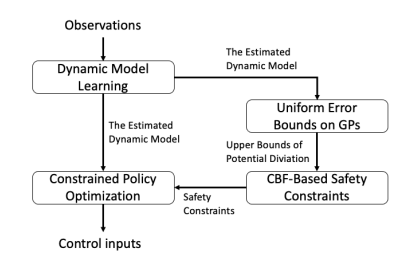
\includegraphics[scale = 1.1]{Flow.png} \\
We will look at each step of this to come up with the required algorithm, providing mathematical rigor by reproducing key proofs.
\subsection{Dynamic Model Learning}
We are aiming to learn the model $f$, so it makes sense that our training input will be both $x_t$ and $u_t$. Denote $\tilde{x_t} = (x_t, u_t) \in \R^{n + p}$. Our training target needs to account for $v_t$, and so we can denote our training target $\Delta_{t + 1} = x_{t + 1} - x_t + v_t$, with $v$ being Gaussian. Let $\Sigma_v$ denote the diagonal matrix, with each entry representing the standard deviation of $v_t$. Since we are in a model based environment, we assume that we have access to $m$ safe training data for initialization. At each step, we would have done more exploration, and added a new input target pair to our training set. As a result, we can denote our training set $\{(\tilde{x_i}, y_i)\}_1^N$ for $N = m + t$ and $y_i = \Delta_i$. Also denote $\Tilde{\vec{X}}$ as the concatenation of the $N$ training inputs. We want to calculate, for arbitrary $x_t$, the value $x_{t + 1} = x_t + \Delta_{t + 1} - v_t$. With this setup, we know $\Delta_{t + 1}$ is Gaussian, with mean and variance given below: 
\begin{equation}
    \E[\Delta_{t + 1}] = \vec{k_*}^T(\vec{K} + \Sigma_v^2\vec{I})^{-1}\vec{y}
\end{equation}
\begin{equation}
    \Var[\Delta_{t + 1}] = k_{**} - \vec{k_*}^T(\vec{K} + \Sigma_v^2\vec{I})^{-1}\vec{k_*}
\end{equation}
Let $k$ denote a kernel function. Then, $\vec{k_*} = k(\Tilde{\vec{X}}, \tilde{x_t}), k_{**} = k(\tilde{x_t}, \tilde{x_t})$ and $\vec{K}$ is the matrix with $K_{ij} = k(\tilde{x_i}, \tilde{x_j})$ (Gram matrix) Now that we have the distribution, including the variance, we can use this for the next step
\subsection{Uniform Error Bounds on GPs}
We have now learned the model as best we can up to the given time step, and importantly for this section, come up with the variance that this model sees. This is used to come up with an error bound on the Gaussian process. This assumes we use a Lipschitz kernel function. Given that, we can come up with an error bound $\eps_{t + 1}$ such that for probability parameter $\delta$ we have \begin{equation}
    P(\length{\tilde{x}_{t + 1} - x_{t + 1}} \leq \eps_{t + 1}, \forall x_{t + 1}) \geq 1 - \delta
\end{equation}
Calculating the exact value of $\eps_{t + 1}$ can be done through a computationally simple formula \cite{lederer2019uniform} but expressing it and explaining the reasoning behind it is notationally and mathematically very dense and not relevant to the topic at hand. What is important is that it is inversely related to the number of training samples $N$ and the probability parameter $\delta$.
This result can also be immediately extrapolated to give 
\begin{align}
    \length{f(x_t, u_t) - \hat{f}(x_t, u_t)} \leq \eps_{t + 1}\\
    \length{B(x_{t + 1} - B(\tilde{x}_{t + 1})} \leq L_B\eps_{t+1}
\end{align} where $\hat{f}$ represents the learned model, and $L_B$ is the Lipschitz constant of $B$. Thus, we now have bounds on the CBF, and the model, and we can use these to come up with the safety constraints.
\subsection{CBF-Based Safety Constraints} 
Since we have known amounts of uncertainty in the problem, we need to modify our CBFs to account for this. The authors did this by defining Uncertainty Tolerant Control Barrier Functions (UTCBFs) which are designed to account for the variance. They are defined by two criteria, given below. For ease of notation, let $B_t$ denote $B(x_t)$. The criteria are \begin{align}
    B_0 \geq 0 \\
    \sup_u\{ \E[(B(\hat{f}(x_t, u_t)) + v_t)|\mathcal{F_t}]\} \geq L_B\eps_{t + 1} + (1 - \gamma)B_t + \beta
\end{align}
Here, $\beta$ and $\gamma$ are chosen such that $\beta \geq 0, \gamma \in (0, 1], B_0 \geq \beta/\gamma$. $\mathcal{F_t}$ is used to denote a knowledge base of the observations of $x, u, v$, like in a martingale. \\
This definition allows us to give a safety guarantee when the barrier function of the safe set satisfies this condition. If there exists a UTCBF $B$ for the system as given in equation 2, then as long as we choose $u_t$ such that \begin{equation}
    \E[B(\hat{f}(x_t, u_t) + v_t] \geq L_B\eps_{t + 1} + (1 - \gamma)B_t + \beta
\end{equation} then $\Pr[B_t \geq 0] \geq 1 - \delta$ which is equivalent by definition to the constraint as specified by equation 3. \\
The proof of this statement employs the martingale like structure of the second criterion for being a UTCBF to come up with random processes based on $B$ that are supermartingales, then using Doob's martingale inequality to prove the probability of $B_t$ being negative can be made negligibly small. The basic structure of the proof involves showing that $u_t$ satisfying equation 11 also satisfies \begin{equation}
    \E[B_{t + 1}|\mathcal{F}_t] \geq (1 - \gamma)B_t + \beta
\end{equation} as long as the error bound from equation 8 is satisfied. Then, we show that if $u_t$ satisfies equation 12, then it must imply that \[\Pr[\inf_t(B_t) < 0]\] can be made negligibly small, completing the proof, since that implies $B_t \geq 0$ for all $t$. We note that the way the error bound is set up, it is very high when the size of the training set is small. So, in the initial exploration phase where not much is known, very few values of $u_t$ can satisfy the constraint of equation 11. However, as we repeat the process over many time steps, and expand our data set, $\eps$ will reduce, and our choice of $u_t$ will become less restricted by safety.
\subsection{Safety Constrained Policy Optimization}
With this work, we can return to our optimization problem in equation 3. We are now able to replace the unspecified constraint $\Pr[x_t\in C, \forall t] > 1 - \delta$ with the concrete $\E[B(\hat{f}(x_t, u_t) + v_t] \geq L_B\eps_{t + 1} + (1 - \gamma)B_t + \beta$. We can use the process set out in the flow to solve this optimization problem, with the actual optimization being done using gradient based, constrained, non-convex optimizers, like Sequential Quadratic Programming (SQP): \\
\begin{algorithmic}[1]
    \State initialize $\theta$ as random
    \State initialize training set with $m$ training data
    \While{not converged}
    \State Learn $\hat{f}(x_t, u_t)$
    \State Calculate $\eps_{t + 1}$
    \State Compute UTCBF and safety constraints
    \State Use the optimizer to calculate gradient update for new $\theta$
    \State Using the new theta, calculate $u_t = \pi(x_t, \theta)$ and add to the training set
    \EndWhile
    \State Return $\theta$
\end{algorithmic}
\subsection{Results}
The authors tested their implementation on the cart pole and inverted pendulum environments provided by Open AI, and compared their results to modern RL algorithms, and other CBF based systems. The RL algorithm used as the benchmark was PILCO \cite{deisenroth2011pilco} which is a widely used algorithm that forms the basis of the model learning that the authors do in their own approach for UTCBF-RL. They were compared based on performance in the cartpole system. The CBF based algorithms used as benchmarks were the model free TRPO-CBF and DDPG-CBF discussed in section 3. They were compared on the inverted pendulum environment. It was found that UTCBF-RL achieved similar, if not slightly better, rewards to these other systems: \\\\
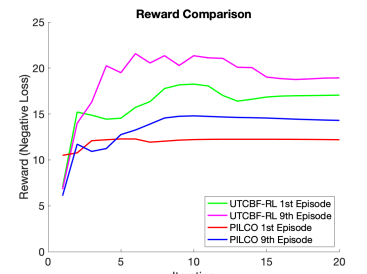
\includegraphics[scale = 0.8]{RewardComparison.png}
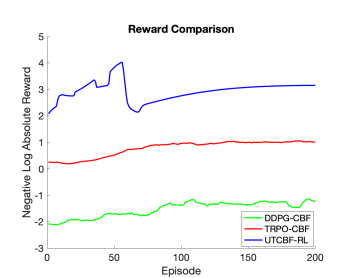
\includegraphics[scale = 0.8]{RewardComparison-CBF.png}\\\\
The raison d'etre for this project, however, was the need for safety, and so that forms the key metric to evaluate it on. It performs very well, as can be seen in the figures below.\\
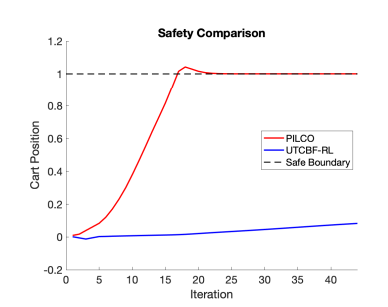
\includegraphics[scale = 0.8]{SafetyComparison.png}
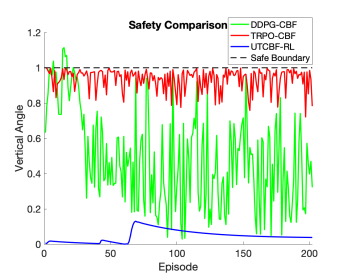
\includegraphics[scale = 0.85]{SafetyComparison-CBF.png}\\
The PILCO algorithm, which makes no consideration for safety, quickly violates the defined safe range in the cart pole environment, while UTCBF-RL stays well away from it. Even in the Pendulum environment, when compared to other modern CBF approaches to RL, this method performs safer, with much less risk and variance, right from the start staying distant from the safety boundary. This shows that the algorithm is making full use of the extra information it is provided by having a model. 
\subsection{Extensions}
The most important extension for this work is to find out convergence rates. While the algorithm has achieved good results in small examples, which shows promise, a better analysis of the time scale over which this algorithm is likely to converge would lend it a lot of confidence for real world applications. It is also an open question whether this can be extended to more complex dynamic systems than the relatively simple, though still powerfully flexible, set up by equation 2.
\section{Further Reading}
Although the wedding of Control Barrier Functions and Reinforcement Learning is a relatively new one, interesting forays have already been made into the field. There are several interesting approaches to combine these two fields beyond the two papers this report focuses on. Here, I will list a few of the most interesting. Marvi and Kiumarsi in their 2021 paper try to reduce the number of interventions the CBF is needed to make for the model-free setting by incorporating it into the cost function itself \cite{marvi2021safe}. Ma et al. try to incorporate a different kind of CBF to the model based setting. Their CBF is based on the distance to the safety boundary and achieves faster convergence, and very few (though not 0) constraint violations \cite{ma2021model}. EMama et al. also approach model based learning with a different variation of CBFs, this time Robust CBFs or RCBFs that generalize the function to work with different kinds of systems \cite{emam2021safe}. Choi et al. combined CBFs with the very similar concept of Control Lyapunov Functions to constrain their (model free) RL algorithm, and were able to achieve safe and stable walking for a bipedal robot \cite{choi2020reinforcement}
\newpage
\bibliography{citations}
\bibliographystyle{ieeetr}
\end{document}